\documentclass{sasbase}

\usepackage[ngerman]{babel}
\usepackage{booktabs}
\usepackage{graphicx}

\begin{document}

\onecolumn
\title{Wahlergebnis - Detail}
\place{Ludwigsburg}
\datum{01. Februar 2017}
\edition{1}

\mytitle

\setlength{\parindent}{0mm}
\setlength{\parskip}{2mm}
\renewcommand{\arraystretch}{1.3}

\section{Präsidentschaftswahl}

David Schwarz wurde knapp mit 5\% bzw. 32 Stimmen Vorsprung gegenüber Paula-Francesca Pompei als Präsident Goethopias gewählt.

\begin{center}
    \begin{tabular}{ |p{3cm}||p{3cm}|p{3cm}|p{3cm}|p{3cm}|  }
     \hline
     \multicolumn{5}{|c|}{Präsidentschaftskandidaten} \\
     \hline
     Kategorie & Aylin Bozcali  & Paula-Francesca Pompei & David Schwarz & Ungültig\\
     \hline
     Stimen   & 87    & 287 &   319 & 11 \\
     Prozent &  12,3  & 40,7   & 45,4 & 1,6 \\
     \hline
    \end{tabular}
\end{center}


\section{Parteienwahl}

Bei der Parteienwahl verteilten sich die Stimmen auf viele kleine Parteien, von denen
einige an der 5\%-Hürde scheiterten. Deshalb hat keine Partei eine Mehrheit und es muss
mindestens eine Koalition aus 3 Parteien gebildet werden.

\vspace{5mm}
\begin{tabular}{ |p{3cm}||p{1cm}|p{1cm}|p{1cm}|p{1cm}|p{1cm}|p{1cm}|p{1cm}|p{1cm}|p{1cm}|p{1cm}|p{1.2cm}|  }
     \hline
     \multicolumn{12}{|c|}{Parteien} \\
     \hline
     Kategorie & DB & DGP & EAP & FiP & GGP & KitKat & KKP & LSD & MIG & PfG & Ungültig\\
     \hline
     Stimen   & 20 & 20  & 123 & 51 & 15 & 76 & 66 & 206 & 54 & 62 & 11 \\
     Anteil in \%  & 2,8 & 2,8  & 17,5 & 7,2 & 2,1 & 10,8 & 9,4 & 29,3 & 7,7 & 8,4 & 1,6 \\
    nach 5\%-Hürde  & 0 & 0 & 19,3  & 8,0 & 0 & 11,9 & 10,3 & 32,3 & 8,5 & 9,7 & 1,6 \\
     \hline
      \hline
     Sitze & 0 & 0 & 6 & 2 & 0 & 4 & 3 & 10 & 3 & 3 & 0\\
     \hline
\end{tabular}

\begin{center}
		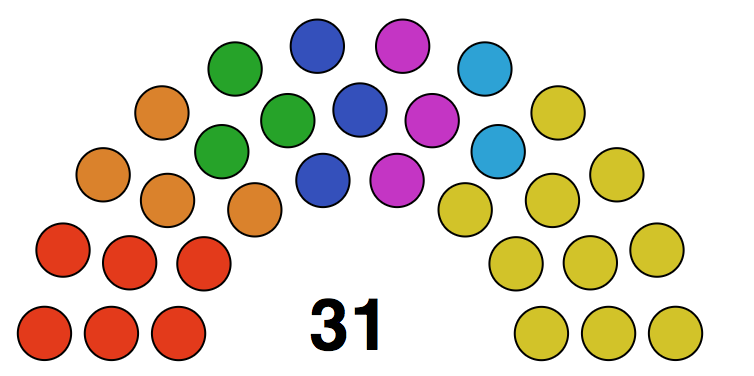
\includegraphics[width=8cm]{parliament.png}
	\end{center}
\newpage

\section{Abgeordnetenliste}

Die Abgeordnetenliste ist noch nicht amtlich und ergibt sich vorläufig aus den von den Parteien abgegeben Wahllisten. Die Abgeordneten haben bis zum 19.02. Zeit, ihre Wahl
abzulehnen. In diesem Fall rückt der nächste Abgeordnete auf der Liste nach. 

\begin{center}
    \begin{tabular}{ |p{5cm}|p{3cm}| }
     \hline
     \multicolumn{2}{|c|}{Abgeordneten im Parlament} \\
     \hline
     Name & Partei \\
     \hline
    Amil Mahmutovic & KKP \\
    Aylin Bozcali & FiP\\
    Anna Hofmann & PfG\\
    Chantal Gliem & MIG\\
    Daniel Höfig & MIG\\
    Daniel Wizemann & KitKat\\
    Elisa Heinzelmann & FiP\\
    Felix Wüstner & EAP\\
    Finn Mann & EAP\\
    Hanna Broghammer & LSD\\
    Henrik Möller & LSD\\
    Ina John & LSD\\
    Johanna Frei & LSD\\
    Joseph von Böhmer & EAP\\
    Jule Mangold & LSD\\
    Julia Bach & LSD\\
    Julia Trachtmann & LSD\\
    Justin Hordorkovski & LSD\\
    Klara Digel & KitKat\\
    Lily Timme & KitKat\\
    Linnea Betz & MIG\\
    Louise Acupanda & KKP\\
    Maximilian Reichert & EAP\\
    Nele Jung & PfG\\
    Nikolas Lamparter & EAP\\
    Robin Deines & LSD\\
    Scott Hebach & LSD\\
    Simon Brettschneider & PfG\\
    Stefan Digel & KitKat\\
    Veronika Seltsam & KKP\\
    Young-Sue Shin & EAP\\
    \hline
    \end{tabular}
\end{center}

\end{document}
